\documentclass{article}

\usepackage{amsmath}
\usepackage[margin=3cm]{geometry}
\usepackage{graphicx}
\usepackage{hyperref}
\usepackage{listings}
\usepackage{minted}


\title{
    \textbf{Programming Club}\\
    EV3 Robots \\
    {\small Based on IVR Robotics Assignment}
}
\author{Volker Seeker}
\date{25$^{th}$ October 2017}

\begin{document}
    \maketitle

\setlength{\parskip}{1em}
\setlength{\parindent}{0em}

    \section{Introduction}
    The aim of this problem is to build an control a robot such that it interacts
    with its environment. You will start off easy by going through a few tutorial
    exercises and then slowly build up towards using multiple sensors to navigate
    your robot. We will use EV3 Lego Mindstorms robots 

    \subsection{Responsibility for the Equipment}
    When handing out the equipment, students are required to
    sign to show they have received the EV3 kit. A \pounds5 deposit
    will also be taken for a key to one of the lockers. It
    is the responsibility of the students to take care of the
    equipment and to return a complete kit. The contents of the
    kit will be checked on return. 

    \section{Typical Usage of the EV3 robot}

  The EV3 has been formatted with a version of Linux called EV3DEV (installed on the SD  
  memory card). It can read from the sensors and can command the motors. We will use a python  
  programming interface to control the robot. The following instructions describe
  \begin{enumerate}
      \item how to connect to the robot (aka the brick) 
      \item copy your program to the robot and run it 
      \item some tutorial exercises to become familiar with the robot. 
  \end{enumerate}

  You can find useful details about ev3dev on its project webpage: 
  \url{http://www.ev3dev.org/}

  and the github repository of the python language bindings:
  \url{https://github.com/ev3dev/ev3dev-lang-python}
  
  \subsection{Starting Up the robot}
  \begin{enumerate}
      \item Plug USB into computer and brick 
      \item Press square button on ev3. It boots through to the ev3dev penguin screen and the 
          brickman screen to the main menu (showing file browser, device browser etc) \\
          \textbf{On DICE computer:} 
          \begin{enumerate}
              \item When the ev3 brick boots, the DICE network manager will create the ev3dev 
  network interface with a static ip address
              \item ssh onto the computer: ssh robot@ev3dev. Password: maker 
          \end{enumerate}
      \item You are now connected to the robot 
      \item (When you are finished shut down by pressing the upper right button a few times)
  \end{enumerate}
   
  As a final note, do not remove the SD card from the robot as this will reset some of the settings 
  and will require you to reconfigure them.

  \subsection{Typical Development Cycle:}

  You will develop your code (in python) in a text editor of your choice on your computer. When 
  you want to test it on the robot, you will copy your entire code directory to the robot. This way 
  you can keep your latest files on your computer at all times. (\textbf{Tip: use (git) version control as your code WILL break as it gets more complex})
  \begin{enumerate}
      \item Write code on your computer. (Make sure your scripts are executable (chmod +x test.py))
      \item Copy the code onto the ev3 to test: \textbf{scp -r ivr\_directory robot@ev3dev:/home/robot/}
      \item When you have copied your programs to the ev3 brick you can use its UI screen to run
  the program by selecting it through ‘file browser’. Unplug the USB cable and press the 
  square button on the EV3 to run the program. \\ 
  You can also execute it directly from a terminal over usb to avoid having to 
  reconnect or to easily see terminal printing (\$~python test.py)

  \item It’s ALIVE! The robot will operate autonomously
  \item To interrupt and end a program press the upper right button for about 3 seconds

  \end{enumerate}



  \section{Tutorial Exercises}

  First download the code samples from this location (or use git checkout):\\
  \url{https://github.com/vsee/ivr\_robotics}

  This contains the tutorial scripts. Put it somewhere on your local file system
  and uncompress it if you downloaded the archive file. You can keep working within
  this directory or copy the file you want to reuse for your own implementations.
  We recommend building reusable classes and functions. Do not implement everything 
  in a single sequence of predetermined functions to make bug hunting easier when it 
  eventually breaks. 
  
  \subsection{Explore Basic Operation of Sensors and Motors}

  \begin{enumerate}
    \item Build the simple wheeled vehicle illustrated below. Make sure to connect the switches to 
        numbers and motors to letters, as shown (brick, wheels and two switches)
    \item Connect to the robot as described in ‘Typical Usage’ 
    \item Progressively work through the tutorials in main.py. You can run main.py from either a 
        terminal or through the EV3’s navigation UI. 
        \begin{enumerate}
            \item Open Loop driving 
            \item Turn an LED on and off with a switch 
            \item Drive backwards and forwards using one switch to command each direction 
            \item Build your first python class to keep ‘state’ of robot  
            \item Attach the Ultrasound sensor, read a set of measurements from it and 
                write them to a text file (depending on where you attach it, you might need to
                adapt the sample code)
        \end{enumerate}
  \end{enumerate}

  \begin{center}
    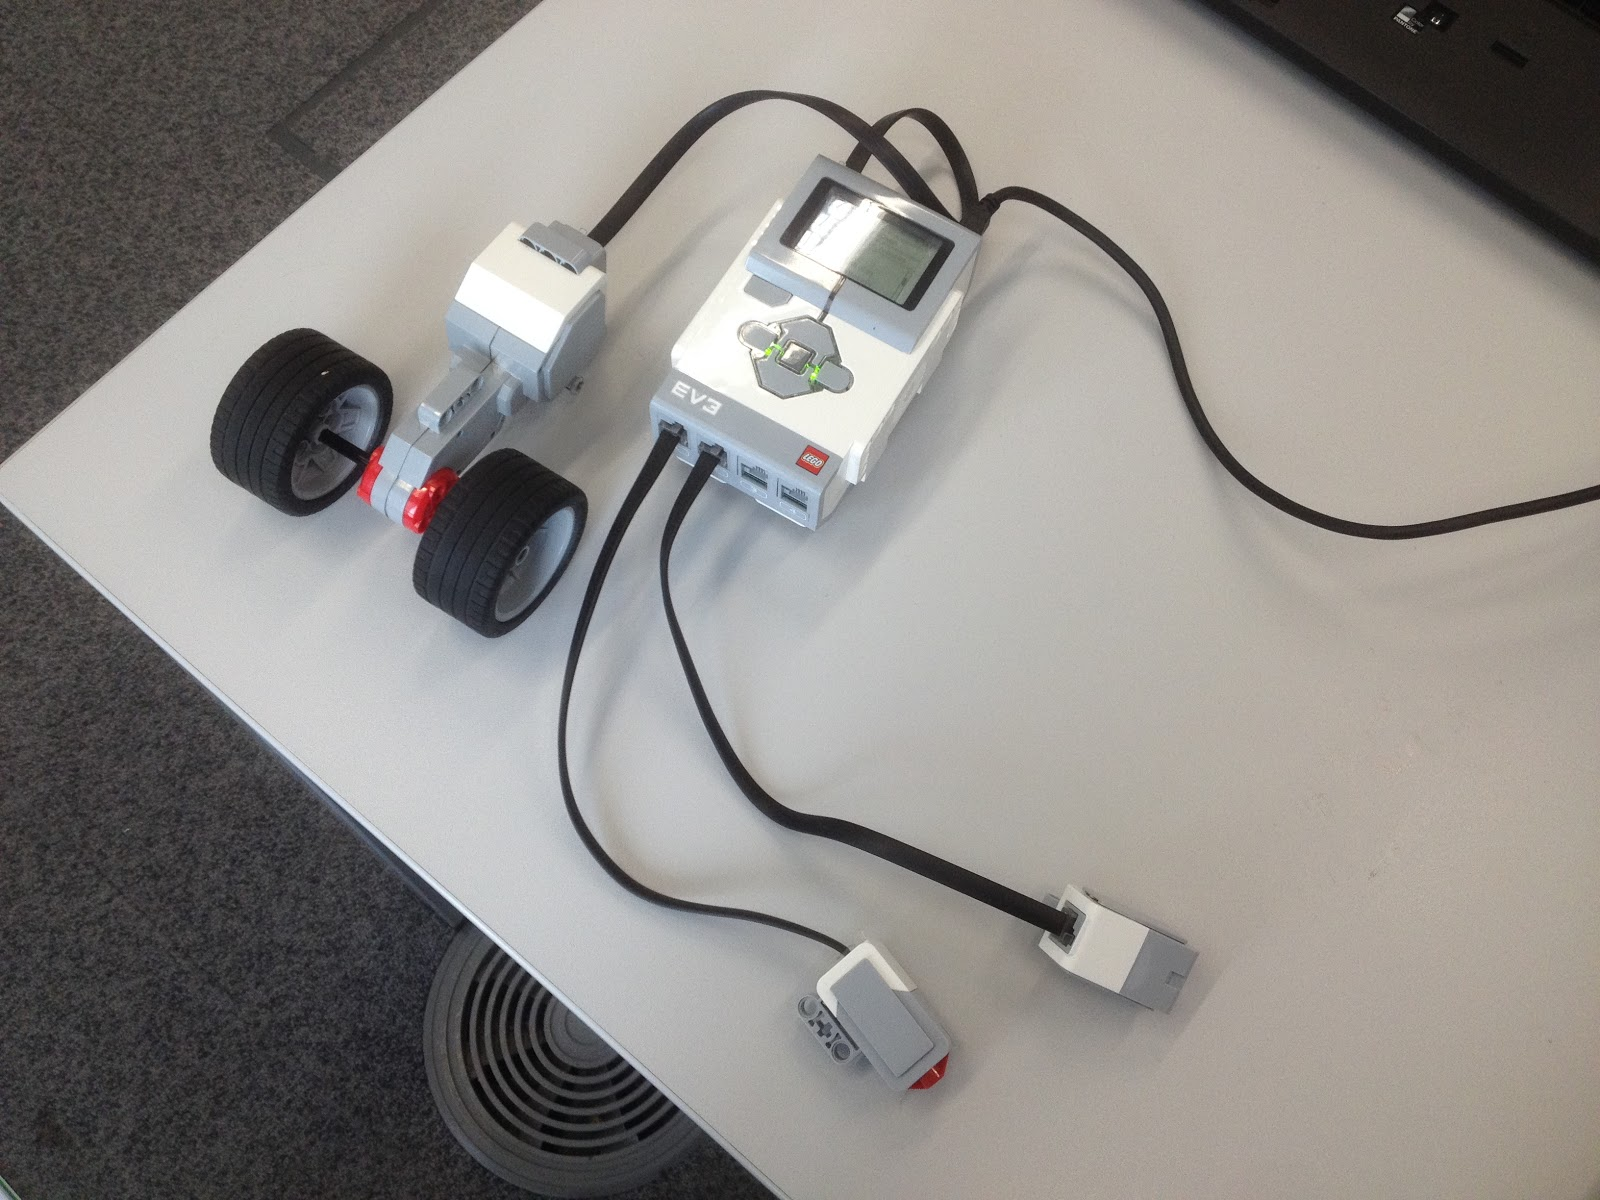
\includegraphics[width=0.5\textwidth]{basic_robot}
  \end{center}


  \section{Problems}

  The following problems will introduce you to various sensors and motors. They are 
  presented in an increasing level of difficulty, but feel free to pick and choose as
  you like.

  \subsection{Driving}
  \begin{enumerate}
    \item build the robot following steps 1 - 40 of the EV3 manual
    \item write a program to make it drive through an obstacle course similar 
        to the one depicted below
    \item measure the time and try to beat your highscore without bumping 
        into any obstacles
  \end{enumerate}

    \begin{center}
        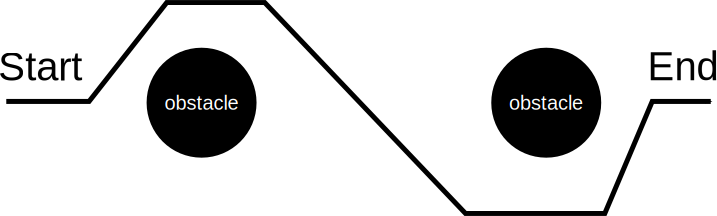
\includegraphics[width=0.7\textwidth]{obstacle_course}
    \end{center}

    Snippet of code to operate the motor and read its encoder value
    (which is the count of the number of counts it turns): \\
 
    \inputminted{python}{../src/python/motor.py}
  
  \subsection{Colour Recognition}
  \begin{enumerate}
      \item attach the colour sensor to your robot (Manual 73 - 76) 
    \item write a program which lets you recognise colours held in front of the sensor (you
        can print a message or make the robot say the colour aloud)
  \end{enumerate}

  Snippet of code to interpret colour sensor readings. Values are between
  0 and 7 with the following interpretations:
  \begin{table}[h]
      \centering
      \begin{tabular}{ c | c | c | c | c | c | c | c | c }
          Colour & none & black & blue & green & yellow & red & white & brown \\
          \hline
          Value & 0 & 1 & 2 & 3 & 4 & 5 & 6 & 7 \\
      \end{tabular}
  \end{table}

  \inputminted{python}{../src/python/colour.py}

  \subsection{Driving between Lines}
  \begin{enumerate}
      \item modify the colour sensor to point downwards (Manual 69 - 72)
      \item make the robot drive until it finds a black line, then make it stop
      \item add more complicated drive pattern, e.g.\ stop at the third line, increase
          robot speed between second and third line, ...
  \end{enumerate}

  \subsection{Driving along Lines}
  \begin{enumerate}
    \item add the gyroscope to your robot (Manual 48 - 53)
    \item write a program that allows your robot to drive along an arbitrary line using 
        the colour sensor to find it and the gyroscope to turn
    \item modify your program, so the robot can drive along broken lines as depicted below
  \end{enumerate}

  \begin{center}
      
\includegraphics[width=0.7\textwidth]{broken_line}
  \end{center}
  
  Snippet of code to print the gyro reading: It returns a number in degrees that
  the sensor has turned: \\
  \inputminted{python}{../src/python/gyro.py}

  \subsection{Avoiding Obstacles}
  \begin{enumerate}
    \item add the ultrasonic sensor to your robot (Manual 42 - 47)
    \item make your robot drive until its sensor finds a close target, then make it stop
    \item modify your program to make the robot drive around and obstacle using the ultrasonic
        sensor and the gyroscope
    \item use the medium motor to build a movable ultrasonic sensor like the one
        in the given video and modify your program to use the new setup \\
        \url{https://www.youtube.com/watch?v=u9SYv3LLMek}
  \end{enumerate}

  Snippet of code to print the ultrasonic sensor reading. It returns millimetres:
  \inputminted{python}{../src/python/sonar.py}

\end{document}
